\section{Atomistic topology}
\label{sec:atomistic}

If you are using \gromacs for generating atomistic configurations, it is possible to directly use the topology file provided by \gromacs (\texttt{topology.tpr}). In this case the \gromacs residue and atom names should be used to specify the \slink{xmlmap}{coarse-grained topology} and \slink{xmlsegments}{conjugated segments}. 

A custom topology can also be defined using an \xml file. Moreover, it s possible to partially overwrite the information provided in, for example, \gromacs topology file. We will illustrate how to create a custom topology file using \dcvt. The structure of \dcvt, together with atom type definitions, is shown in fig.~\ref{fig:dcv2t}. \dcvt has two thiophene (THI) and two dicyanovinyl (NIT) residues. The pdb file which contains residue types, residue numbering, atom names, atom types, and atom coordinates is shown in listing~\ref{list:pdb}.

\begin{figure}[ht]
\centering
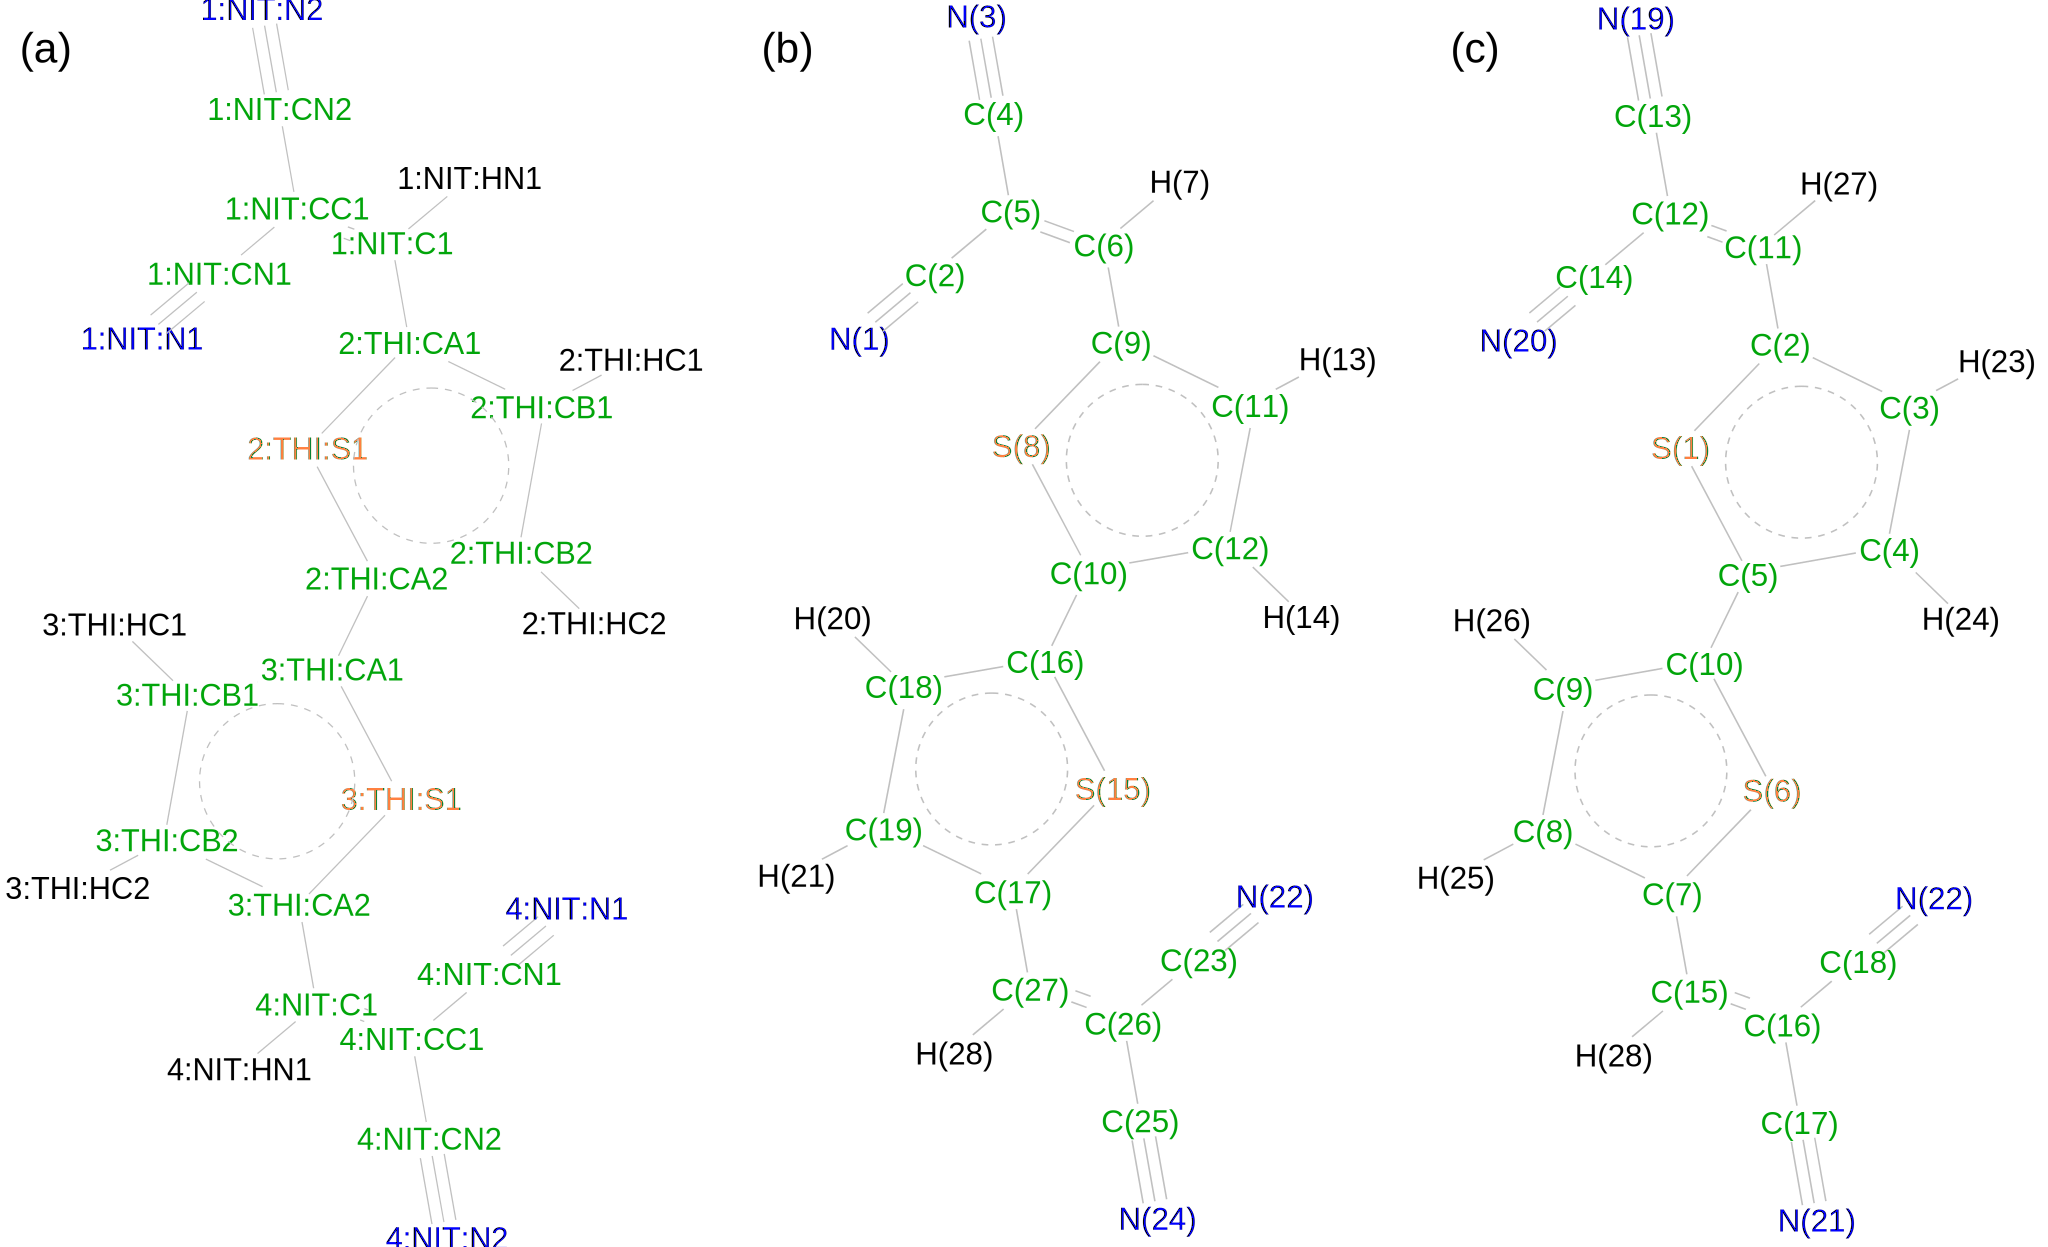
\includegraphics[width=\textwidth]{./fig/chemical_structure/dcv2t}
\caption{\small (a) \dcvt with atoms labelled according to \texttt{residue\_number:residue\_name:atom\_name}. 
There are four residues and two residue types: thiophene (THI) and dicyanovinyl (NIT). The corresponding pdb file is shown in listing~\ref{list:pdb}. 
Atom numbering is used to split conjugated segments on rigid fragments and to link atomistic ((b) from GROMACS topology) and quantum descriptions (c).}
\label{fig:dcv2t}
\end{figure}

\lstinputlisting[
  language=XML,
  basicstyle=\ttfamily\footnotesize,
  stringstyle=\ttfamily\footnotesize,
  showstringspaces=false,
  frame=lines,
  label=list:pdb, 
  morekeywords={HETATM,THI,NIT},
  caption={ pdb file of \dcvt.}]%
{./input/dcv2t/dcv2t.pdb}
\vfill